%Modify the relative path accordingly
%HU, Pili
%Create: 20120330
%Modify: 20120330
%The unified entry to include in my tutorial series

%HU, Pili
%Create: 20110910
%Modify: 20120330
%purpose of this file is to gather commonly used
%mathematical abbreviations, to speed up writing
%notes

\documentclass[11pt,a4paper]{article}
\usepackage[utf8x]{inputenc}
\usepackage{ucs}
\usepackage{amsmath}
\usepackage{amsfonts}
\usepackage{amssymb}
\usepackage{amsthm}
\usepackage{url}
\usepackage{graphicx}

\usepackage{fancyhdr}
\pagestyle{fancy}
\fancyhead{}

%=====Calculus======
%the following commands are not originated by me
%I pick them from http://www-solar.mcs.st-and.ac.uk/~clare/Latex/
%the following line controls the style of patial derivative
%1), use \dfrac, height is larger, looks good. 
%2), use \frac, also work, but space looks limited. 
\newcommand{\myfrac}[2]{\dfrac{#1}{#2}}
\newcommand{\diff}[2]{\myfrac{{\rm d}#1}{{\rm d}#2}}
\newcommand{\ndiff}[3]{\myfrac{{\rm d}^{#3}#1}{{\rm d}#2^{#3}}}
\newcommand{\pdiff}[2]{\myfrac{\partial #1}{\partial #2}}
\newcommand{\npdiff}[3]{\myfrac{\partial^{#3} #1}{\partial #2^{#3}}}
\newcommand{\e}[1]{\ensuremath{{\rm e}^{#1}}}
\newcommand{\ldiff}[2]{\ensuremath{{\rm d}#1/{\rm d}#2}}
\newcommand{\lpdiff}[2]{\ensuremath{\partial#1/\partial#2}}
\newcommand{\lnpdiff}[3]{\ensuremath{\partial^{#3}#1/\partial#2^{#3}}}
\newcommand{\dif}[1]{\mathrm{d}#1}

%20120330
%The reason I don't copy the original file as a whole
%is that it contains too many individually preferred 
%definitions. 
%
%I start with those basic symbols and adapt them in use. 

%=====Matrix======
\newcommand{\tr}[1]{\mathrm{Tr}\left[#1\right]}
\newcommand{\tran}[1]{#1^\mathrm{T}}
%The following shorthand of matrix may be convenient. 
%However, it is so short that I'm worried it may 
%collide with something else. I don't use at present.
%\newcommand{\m}[1]{\mathbf{#1}}
\newcommand{\adj}[0]{\mathrm{adj}}

%=====Theorem definitions=====
\newcounter{mytheoremorder}
\newtheorem{mydef}{Definition}
\newtheorem{myaxm}{Axiom}
\newtheorem{mythm}[mytheoremorder]{Theorem}
\newtheorem{myprop}[mytheoremorder]{Proposition}
\newtheorem{myex}{Example}

%=====Optimization====
\DeclareMathOperator*{\argmax}{arg\,max}
\DeclareMathOperator*{\argmin}{arg\,min}
\newcommand{\maximize}[0]{\mathrm{Maximize~}}
\newcommand{\minimize}[0]{\mathrm{Minimize~}}

%=====Probability====
\newcommand{\E}[0]{\mathbb{E}}
\newcommand{\var}[0]{\mathrm{Var}}
\newcommand{\cov}[0]{\mathrm{Cov}}

%=====Quick and Unified Reference====
%20120505
%Usage: \eq{\ref{xxx}}
%The reason I keep "\ref" away from definition, 
%and let user type it every time is that: 
%currently I'm working on Texmaker, and it can 
%trigger a selection panel when the sequence 
%"\ref" is found. Maybe further configuration of 
%texmake can make it do the same thing when the 
%following self-defined sequence is detected.
%This is left for future work. 
\newcommand{\req}[1]{\textbf{Eq~{#1}}}
\newcommand{\rfig}[1]{\textbf{Fig~{#1}}}
\newcommand{\rtbl}[1]{\textbf{Tbl~{#1}}}
\newcommand{\rpg}[1]{\textbf{P~{#1}}}
\newcommand{\rsec}[1]{\textbf{Section~{#1}}}


\usepackage{algorithm}
\usepackage{algorithmic}
\floatname{algorithm}{Algorithm}
\renewcommand{\algorithmicrequire}{\textbf{Input:}}
\renewcommand{\algorithmicensure}{\textbf{Output:}}

\usepackage{subfigure}

\fancyhead[LO,LE]{HU, Pili}
\fancyhead[RO,RE]{Spectral Clustering Survey}

%This usually doesn't need modification 
\author{HU, Pili\thanks{hupili [at] ie [dot] cuhk [dot] edu [dot] hk}}

%Modify them accordingly===
\title{Spectral Clustering Survey}
\date{May 14, 2012\thanks{Last compile:\today}}

\begin{document}

\maketitle
%>============================================
\begin{abstract}
	Abstract. Sources can be found in \cite{hu2012-spectral2hop}. 
\end{abstract}
%<=======Abstract ENd=========================

%>============================================
\pagebreak
\setcounter{tocdepth}{2}
\tableofcontents
\pagebreak
%<=======TOC ENd==============================



\section{Introduction}
\label{sec:introduction}

Spectral Clustering(SC) was used in several disciplines long ago. 
For example, computer vision\cite{shi2000normalized}, load balancing
\cite{hendrickson1993multidimensional}, electronics design
\cite{hadley1992efficient}, etc.  Spectral Embeding(SE) was 
also widely discussed in the community\cite{brand2003unifying}. 
Outside spectral community, the machine learning community also 
developed many linear or non-linear Dimensionality Reduction(DR) methods, 
like Principal Component Anslysis (PCA), Kernel PCA (KPCA)\cite{scholkopf1998kpca}, 
Locally Linear Embedding (LLE)\cite{roweis2000lle}, etc. 
Other technique like Multi-Dimensional Scaling(MDS) was successfully 
used in computational psychology for a very long time\cite{borg2005modern}, 
which can be viewed as both "embedding" or "dimensionality reduction".


According to our survey, although those methods target at different problems
and are derived from different assumptions, they do share a lot in common. 
The most significant sign is that, the core procedure involves 
eigenvalue decomposition or singular value decomposition, aka "spectral". 
They all involve an intermidiate step of embedding high-dimensional / 
non-Euclidean / non-metric points into a low-dimensional Euclidean space
(although some do not embed explicitly). In this case, we categorize all 
these algorithms as Spectral Embedding Technique(SET). 

\subsection{A Sample Spectral Clustering Algorithm}

%%Following is just an example copied from:
%%http://en.wikibooks.org/wiki/LaTeX/Algorithms_and_Pseudocode
%\begin{algorithm}                      % enter the algorithm environment
%\caption{Calculate $y = x^n$}          % give the algorithm a caption
%\label{alg1}                           % and a label for \ref{} commands later in the document
%\begin{algorithmic}                    % enter the algorithmic environment
%    \REQUIRE $n \geq 0 \vee x \neq 0$
%    \ENSURE $y = x^n$
%\end{algorithmic}
%\end{algorithm}

There are many variations of SC. They all work under certain conditions
and researchers don't have a rule of thumb so far. Before we analyze their
procedure and justification, we present a simple but workable sample 
algorithm(\ralg{\ref{alg:sc_sample}}). 

\begin{algorithm}[htb]
	\caption{Sample Spectral Clustering}
	\label{alg:sc_sample}
	\begin{algorithmic}[1]
		\REQUIRE Data matrix $X = [x_1, x_2, \ldots, x_N]$;  
		Number of Clusters $K$. 
		\ENSURE Clustering $\{C_i\}$: $C_i \in V$ 
			and $\cap_i C_i = \emptyset$
			and $\cup_i C_i = V$. 
		\STATE Form adjacency matrix $A$ within $\epsilon$-ball.
		\STATE Solve $A = U \Lambda \tran{U}$, indexed according 
		the eigenvalue's magnitude. 
		\STATE $Y \leftarrow$ first $K$ columns of U. 
		\STATE Cluster $Y$'s rows by K-means. 
	\end{algorithmic}
\end{algorithm}

In \ralg{\ref{alg:sc_sample}}, the $\epsilon$-ball adjacency graph is 
constructed as follows. First create one vertex for each data point. 
If for two points $i,j$ satisfy $||x_i-x_j|| < \epsilon$, connect 
them with an edge. In this simple demonstration, we consider an unweighted
graph, i.e. all entries of $A$ are 0(disconnected) or 1(connected). 

\begin{figure}
	\centering
	\subfigure[Data Scatter Plot]{
		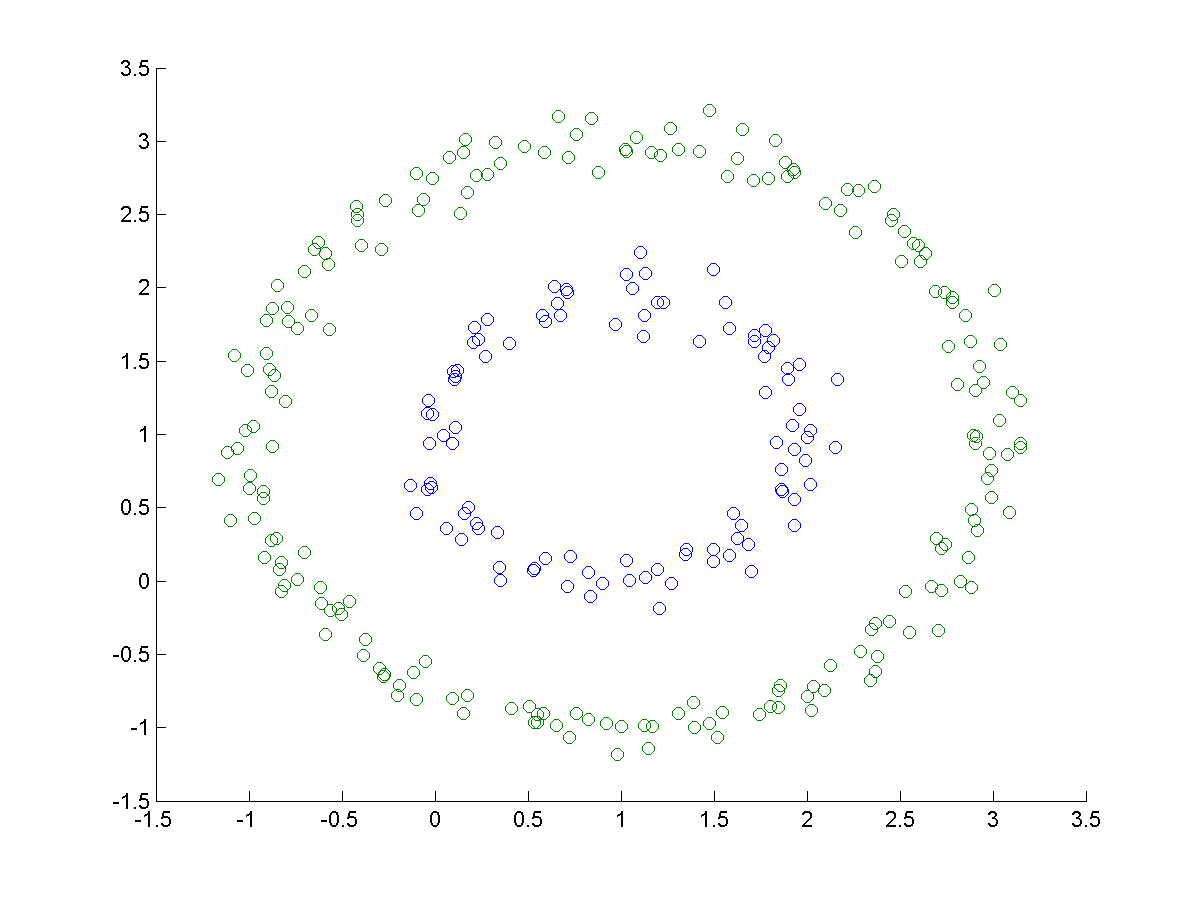
\includegraphics[width=0.4\textwidth]{../plot/sc_sample_scatter.png}	
		\label{fig:ssc_data}
	}
	\subfigure[Standard K-means]{
		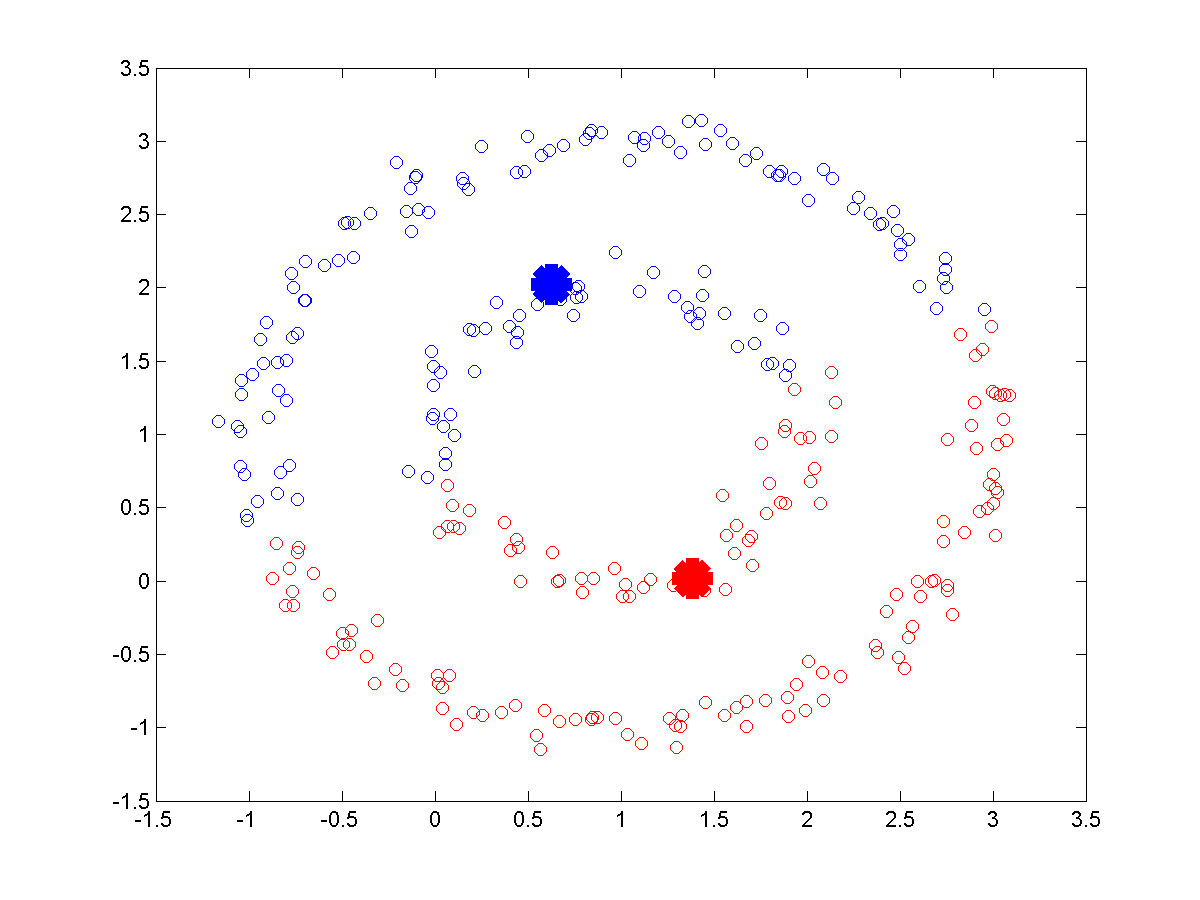
\includegraphics[width=0.4\textwidth]{../plot/sc_sample_kmeans.png}	
		\label{fig:ssc_kmeans}
	}
	\subfigure[Adjacency Graph]{
		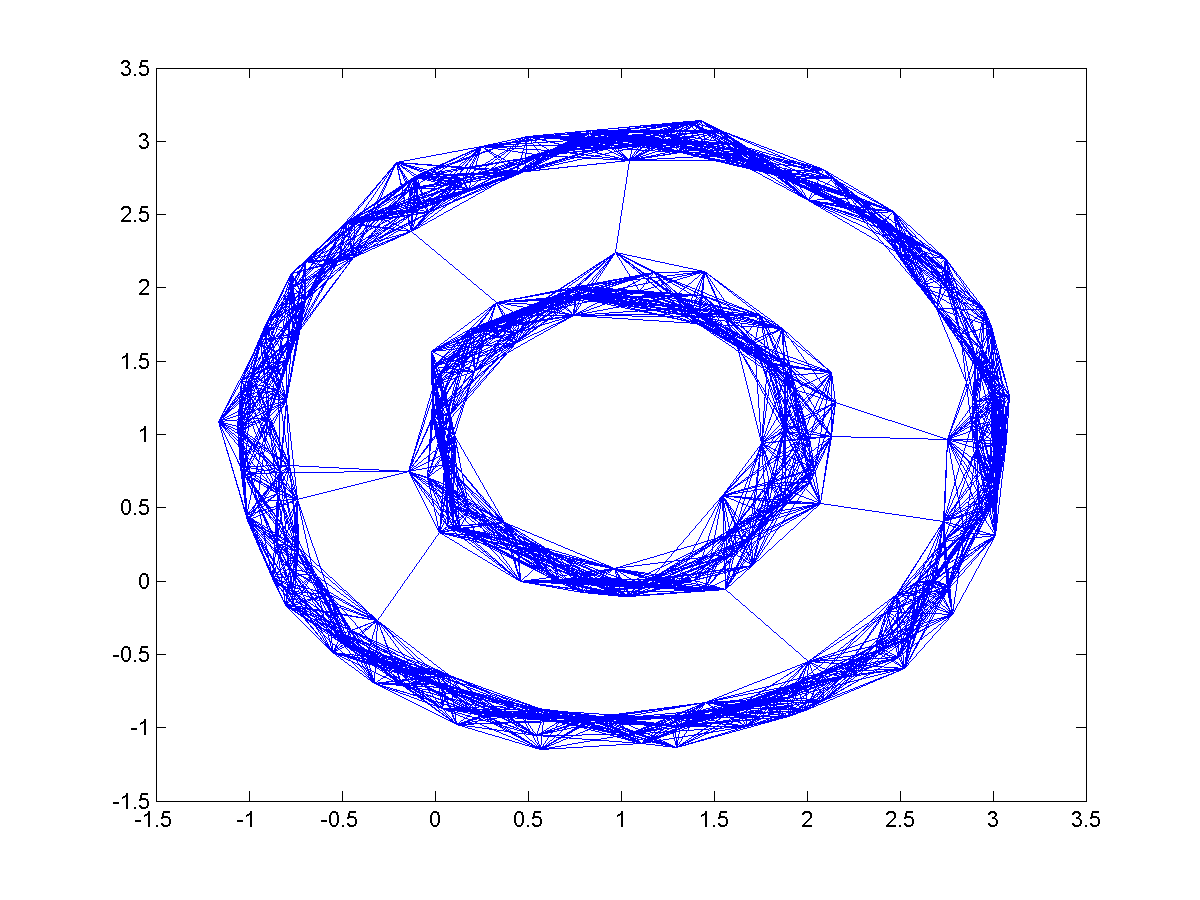
\includegraphics[width=0.4\textwidth]{../plot/sc_sample_adj.png}	
		\label{fig:ssc_adj}
	}
	\subfigure[Sample SC Algorithm]{
		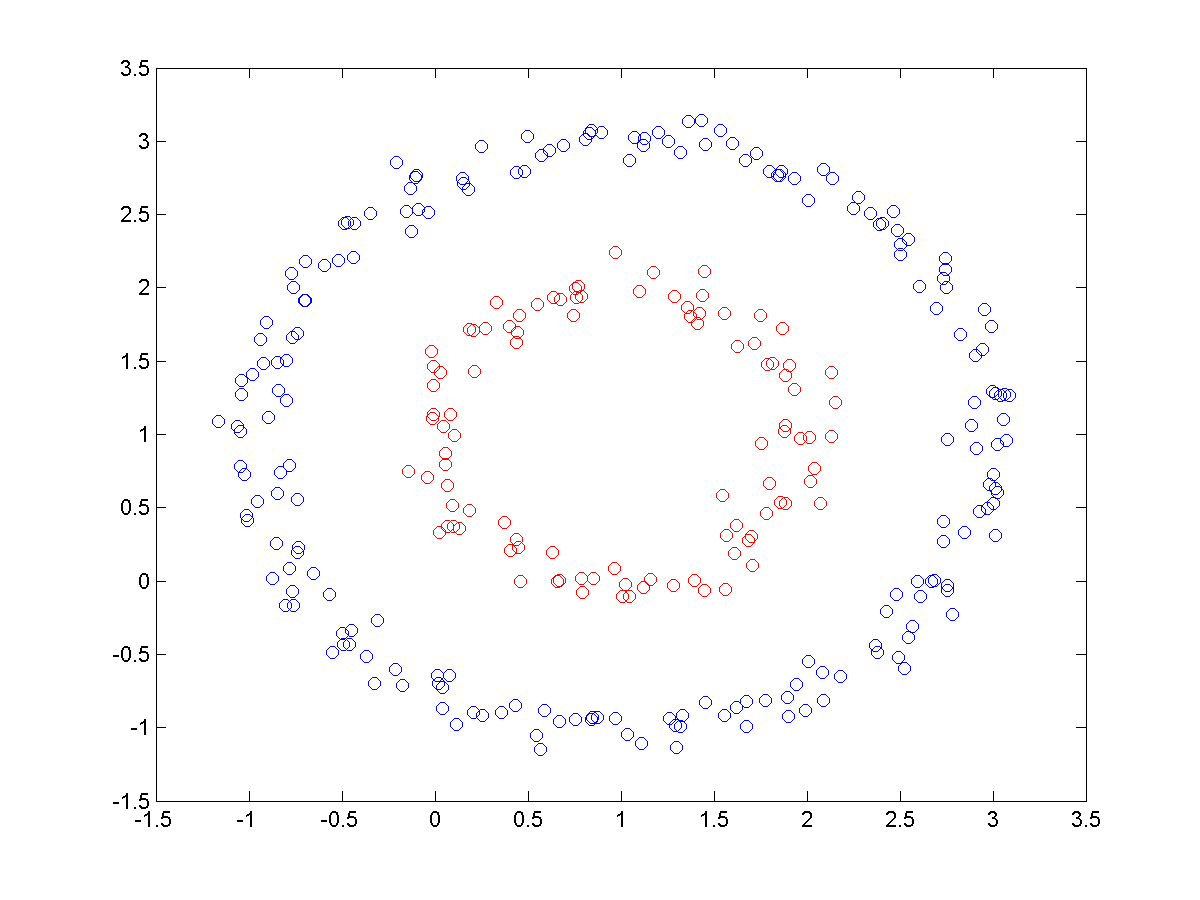
\includegraphics[width=0.4\textwidth]{../plot/sc_sample_sc.png}	
		\label{fig:ssc_sc}
	}
	\caption{Demonstration of Sample SC Algorithm}
	\label{fig:ssc_demo}
\end{figure}

\rfig{\ref{fig:ssc_demo}} demonstrates the result of our sample SC algorithm, 
compared with standard K-means algorithm. 
\rfig{\ref{fig:ssc_data}} shows the scatter plot of data. 
It is composed of one radius 1 circle and another radius 2 circle, 
both centered at (1,1). 
\rfig{\ref{fig:ssc_kmeans}} shows the result of standard K-means
working on Euclidean distance. 
\rfig{\ref{fig:ssc_adj}} shows the graph representation, where 
the adjacency graph is formed by taking a $\epsilon$-ball and 
$\epsilon=0.7$ in the example. 
\rfig{\ref{fig:ssc_sc}} shows the output of \ralg{\ref{alg:sc_sample}}. 
It's obvious that standard K-means algorithm can not correctly cluster 
the two circles. This is a known major weakness of K-means(in Euclidean): 
When clusters are not well separated spheres, it has difficulty recovering 
the underlying clusters. Although K-means works for this case 
if we transform the points 
into polar coordinate system(see \cite{hu2012-spectral2hop} for code), 
the solution is not universal. However, in this example, our sample SC 
algorithm can separate the two clusters, probably because the eigenvectors
of adjacency matrix convey adequate information. 

A precaution is that \ralg{\ref{alg:sc_sample}} does not always work even 
in this simple case. Nor have we seen this algorithm from formally published works
(so far), let alone justifications. This algorithm is only to show the flavour 
of spectral clustering and it contains those important steps in other
more sophisticated algorithms. Readers are recommended to learn 
von Luxburg's tutorial\cite{von2007tutorial} before reading the following sections. 
Since that paper is very detailed, we'll present overlapping topics 
concisely. 


\subsection{Linear Algebraic Properties}

\section{Spectral Clustering Framework}

\subsection{Metric Formulation}

\subsection{Spectral Embeding}

\subsection{Clustering}


\section{Spectral Clustering Justification}
\label{sec:justification}

\subsection{Random Walk}
[von]

\subsection{Normalized Cut}
[shi]

\subsection{Ratio Cut}
[von]

\subsection{Conductance}
[von]

\subsection{Matrix Perturbation}
[andrew ng]

\subsection{Low Rank Approximation}
[matthew brand]

\subsection{Density Estimation View}
[mo chen, 2010]

\subsection{Commute Time}
[jihun ham, kernel]. 
view pseudo inverse of graph Laplacian by commute times on graphs. 

\subsection{Polarization}
[m. brand] unifying view... 

\section{Other Spectral Like Embedding}
\label{sec:nldr}

\subsection{MDS}

\subsection{isomap}

\subsection{Laplacian Eigenmap}

\subsection{Hessian Eigenmap}

\subsection{PCA}

\subsection{LLE}

\subsection{Kernel PCA}

\subsection{Kernel Framework}

\subsection{Graph Framework}


\section{Conclusion}
\label{sec:conclusion}



%>============================================
\section*{Acknowledgements}
\addcontentsline{toc}{section}{Acknowledgements}

%<=======Acknowledgements ENd=================

%>============================================
\addcontentsline{toc}{section}{References}
\input{../reference/gen_bib.bbl}
%<=======Bibliography ENd=====================

%>============================================
\section*{Appendix}
\addcontentsline{toc}{section}{Appendix}

%<=======Appendix ENd=========================

\end{document}
